\subsection{Channel Model Design}

This section describes the wireless channel model used in the baseline OTFS simulation. The purpose of the channel model is to represent a time-varying multipath propagation environment with both delay and Doppler effects. The same channel generation mechanism is used for OFDM-LMMSE, baseline OTFS, and OTFS-IM so that the performance comparison in Chapter 5 remains consistent.

\subsubsection{Time-Varying Multipath Channel Overview}

In OTFS theory, a time-varying wireless channel can be represented in the delay-Doppler domain by a finite number of propagation paths. Each path is characterized by a delay, a Doppler shift, and a complex channel coefficient. This representation is suitable for OTFS because the transmitted information symbols are first arranged in the delay-Doppler domain before being transformed for transmission.

In the simulation model used in this thesis, the continuous delay-Doppler channel is represented by discrete channel taps. The channel is described by
\begin{equation}
    \{h_i,l_i,\nu_i\}_{i=1}^{P},
\end{equation}
where \(P\) is the number of channel paths, \(h_i\) is the complex fading coefficient of the \(i\)-th path, \(l_i\) is the discrete delay tap, and \(\nu_i\) is the discrete Doppler tap. In this model, \(\nu_i\) denotes a Doppler-tap index on the OTFS grid rather than a physical Doppler frequency in hertz. The Doppler tap is therefore represented as a normalized integer index on the OTFS Doppler grid.

A conceptual representation of the channel model is shown in Fig.~\ref{fig:discrete_multipath_channel}. The transmitted signal is passed through several delayed, Doppler-shifted, and faded propagation paths. The path contributions are then summed and complex additive white Gaussian noise is added.

\begin{figure}[H]
    \centering
    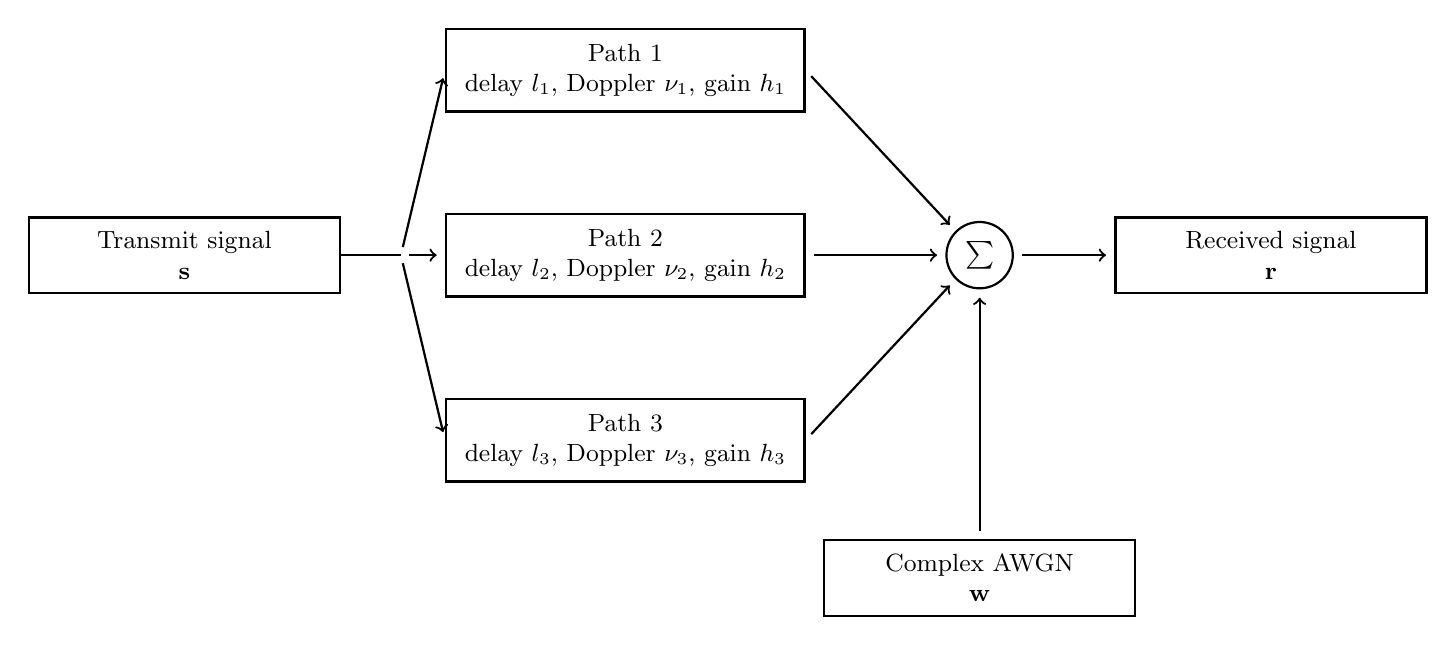
\begin{tikzpicture}[
        block/.style={
            rectangle,
            draw,
            thick,
            align=center,
            text width=3.6cm,
            minimum height=0.9cm,
            font=\small,
            inner sep=5pt
        },
        pathblock/.style={
            rectangle,
            draw,
            thick,
            align=center,
            text width=4.2cm,
            minimum height=1.05cm,
            font=\small,
            inner sep=5pt
        },
        sum/.style={
            circle,
            draw,
            thick,
            minimum size=0.8cm,
            font=\small
        },
        arrow/.style={
            ->,
            thick,
            shorten >=3pt,
            shorten <=3pt
        }
    ]

        \node[block] (input) at (0,0) {Transmit signal\\\(\mathbf{s}\)};

        \coordinate (split) at (2.75,0);

        \node[pathblock] (p1) at (5.6,2.35) {Path 1\\delay \(l_1\), Doppler \(\nu_1\), gain \(h_1\)};
        \node[pathblock] (p2) at (5.6,0) {Path 2\\delay \(l_2\), Doppler \(\nu_2\), gain \(h_2\)};
        \node[pathblock] (p3) at (5.6,-2.35) {Path 3\\delay \(l_3\), Doppler \(\nu_3\), gain \(h_3\)};

        \node[sum] (sum) at (10.1,0) {\(\sum\)};
        \node[block] (noise) at (10.1,-4.1) {Complex AWGN\\\(\mathbf{w}\)};
        \node[block] (output) at (13.8,0) {Received signal\\\(\mathbf{r}\)};

        \draw[thick] (input.east) -- (split);
        \draw[arrow] (split) -- (p1.west);
        \draw[arrow] (split) -- (p2.west);
        \draw[arrow] (split) -- (p3.west);

        \draw[arrow] (p1.east) -- (sum.north west);
        \draw[arrow] (p2.east) -- (sum.west);
        \draw[arrow] (p3.east) -- (sum.south west);

        \draw[arrow] (noise.north) -- (sum.south);
        \draw[arrow] (sum.east) -- (output.west);

    \end{tikzpicture}
    \caption{Discrete time-varying multipath channel model}
    \label{fig:discrete_multipath_channel}
\end{figure}

\subsubsection{Delay and Doppler Tap Representation}

The channel model uses three multipath components, so
\begin{equation}
    P = 3.
\end{equation}
The delay taps are fixed as
\begin{equation}
    \mathbf{l} = [0,1,2],
\end{equation}
which means that the three paths arrive with different discrete delays. These delay taps create delay spread in the received signal.

The Doppler taps are generated randomly for each channel realization. Each Doppler tap belongs to the set
\begin{equation}
    \nu_i \in \{-4,-3,-2,-1,0,1,2,3,4,5\}.
\end{equation}

The Doppler taps introduce time variation through phase rotation across the transmitted samples. A larger absolute Doppler tap produces faster phase variation. Since the Doppler values are represented as discrete indices, the model captures Doppler-induced time selectivity without assigning a specific physical velocity in kilometres per hour.

\subsubsection{Rayleigh Fading Path Coefficients}

Each channel path is assigned a complex fading coefficient. The channel coefficients are modeled as
\begin{equation}
    h_i
    =
    \sqrt{\frac{e^{-l_i}}{2}}
    \left(
    a_i + jb_i
    \right),
    \label{eq:channel_coeff}
\end{equation}
where \(a_i\) and \(b_i\) are independent real Gaussian random variables.

Because \(h_i\) is complex Gaussian, its amplitude follows a Rayleigh fading behavior. The factor \(e^{-l_i}\) introduces a delay-dependent power profile, where paths with larger delays have lower average power. This produces a simple exponentially decaying multipath channel profile.

\subsubsection{Discrete Channel Input-Output Operation}

Let \(\mathbf{s}\) be the transmitted time-domain vector generated by the OTFS transmitter. The channel output is obtained by summing the contribution of all delayed and Doppler-shifted paths. A compact discrete representation is
\begin{equation}
    r[q]
    =
    \sum_{i=1}^{P}
    h_i
    e^{j\phi_i(q)}
    s[q-l_i]
    +
    w[q],
    \label{eq:discrete_channel}
\end{equation}
where \(q\) is the discrete time-sample index, \(l_i\) is the delay tap, \(e^{j\phi_i(q)}\) is the Doppler-induced phase rotation, and \(w[q]\) is the additive noise sample.

The Doppler phase rotation is represented through the exponential term
\begin{equation}
    \exp
    \left(
    j\frac{2\pi}{M}
    q
    \frac{\nu_i}{N}
    \right).
\end{equation}
Each path contribution is then circularly shifted according to its delay tap and weighted by its complex channel coefficient.

Before applying the channel, a cyclic-prefix-like extension is added using the maximum delay tap. After the channel and noise are applied, this prefix part is removed so that the received vector has the same length as the transmitted OTFS frame.

\subsubsection{Additive White Gaussian Noise}

After the multipath channel output is generated, complex additive white Gaussian noise is added. The noise sample is modeled as
\begin{equation}
    w[q]
    =
    \sqrt{\frac{\sigma^2}{2}}
    \left(
    n_{\mathrm{I}}[q] + jn_{\mathrm{Q}}[q]
    \right),
    \label{eq:awgn}
\end{equation}
where \(n_{\mathrm{I}}[q]\) and \(n_{\mathrm{Q}}[q]\) are independent real Gaussian random variables with zero mean and unit variance.

The noise variance \(\sigma^2\) is computed from the selected \(E_b/N_0\) value and the spectral efficiency of the corresponding transmission scheme. Therefore, OFDM-LMMSE, OTFS, and OTFS-IM are evaluated under consistent energy-per-bit conditions.

\subsubsection{Channel Parameters Used in Simulation}

The main channel parameters are summarized in Table~\ref{tab:channel_model_parameters}. These parameters are used consistently across the baseline OTFS system, the OFDM-LMMSE reference, and the OTFS-IM simulations.

\begin{table}[H]
    \centering
    \caption{Delay-Doppler channel parameters used in simulation}
    \label{tab:channel_model_parameters}
    \begin{tabular}{c c c}
        \hline
        Parameter & Symbol & Value \\
        \hline
        Number of channel paths & \(P\) & 3 \\
        Delay taps & \(\mathbf{l}\) & \([0,1,2]\) \\
        Doppler tap range & \(\nu_i\) & \(-4\) to \(5\) \\
        Fading coefficient & \(h_i\) & Complex Gaussian \\
        Fading amplitude & \(|h_i|\) & Rayleigh-type fading \\
        Delay power profile & -- & Exponential decay \(e^{-l_i}\) \\
        Noise model & \(w[q]\) & Complex AWGN \\
        CSI assumption & -- & Known channel parameters at receiver \\
        \hline
    \end{tabular}
\end{table}

\subsubsection{Channel Model Summary}

The channel model used in this thesis is a discrete delay-Doppler multipath Rayleigh fading channel with additive white Gaussian noise. It includes three propagation paths, fixed delay taps, random discrete Doppler taps, and complex Gaussian fading coefficients. This structure is consistent with the OTFS principle that channels with delay and Doppler dispersion can be represented compactly in the delay-Doppler domain.

The model is intentionally controlled rather than fully standardized. It does not assign a specific mobile velocity or use a complete 3GPP channel profile. Instead, it provides a common high-Doppler delay-Doppler fading environment for comparing OFDM-LMMSE, OTFS, and OTFS-IM under the same channel conditions.
